\section{Incontro}

\subsection{Ordine del giorno}
\begin{itemize}
    \item Presentazione MVP;
    \item dimostrazione delle funzionalità dell'MVP;
    \item conslusioni e feedback.
\end{itemize}

\subsection{Discussione}
Sono state presentate le funzionalità principali del prodotto sviluppato (MVP) al proponente, dimostrando come esse soddisfino gli obiettivi prefissati. Il proponente è rimasto ampiamente soddisfatto dalle funzionalià implementate.\ref{fig:email-mvp}
A fine presentazione il proponente ha elencato alcuni punti da migliorare e/o implementare per il prodotto finale (Customer Acceptance), tra cui:
\begin{itemize}
    \item impostare la dashboard delle aree come pagina principale, offrendo un accesso diretto ai lampioni dalla zona selezionata;
    \item inserimento manuale dei guasti: per gli utenti loggati con il ruolo di manutentore, sarebbe opportuno fornire pulsanti che consentano loro di segnalare un guasto come "risolto" in modo da semplificare il processo di manutenzione.
    \item inoltre, si potrebbe implementare una funzione di rilevazione guasti automatica: in caso di mancata risposta entro 5 minuti, il sistema dovrebbe identificare un possibile guasto al sensore e segnalarlo all'utente tramite un LED rosso nella web app. Si potrebbe valutare l'utilizzo delle API di Jira per facilitare la gestione di queste segnalazioni.
\end{itemize}

\subsection{Conferma MVP}

%Allega immagine mvp.jpg
\begin{figure}[H]
    \centering
    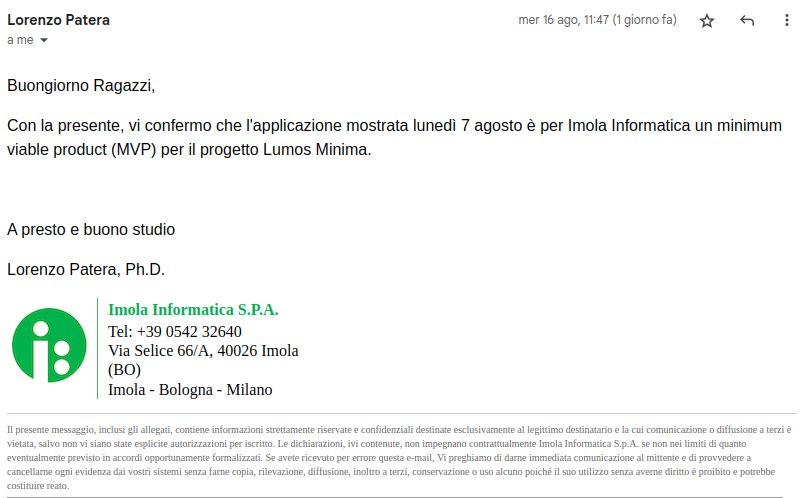
\includegraphics[width=\textwidth]{img/mvp.jpg}
    \caption{Email di conferma del proponente per l'MVP}
    \label{fig:email-mvp}
\end{figure}